\documentclass[tikz, border=0pt]{standalone}
\usepackage{siunitx}
\usepackage{tikz-3dplot}
\usepackage{physics}
\usepackage{amsmath}
\usetikzlibrary{decorations,decorations.markings,decorations.text}

\definecolor{amber}{rgb}{1.0, 0.75, 0.0}
\definecolor{goldmetallic}{rgb}{0.83, 0.69, 0.22}

\begin{document}

\tikzset{>=latex} % for LaTeX arrow head

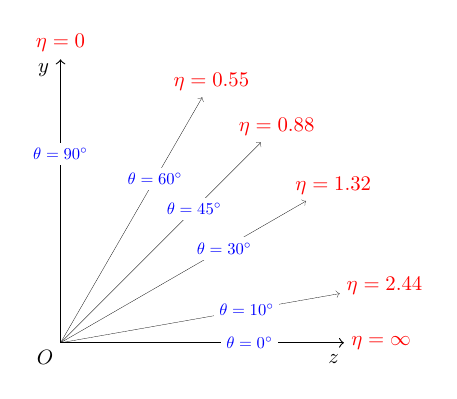
\begin{tikzpicture}[scale=3]
 
    % limits
    %\def\N{4}
    \def\R{1.2}
    
    % axis labels
    \node[scale=0.75,below=5pt,left=2pt] at (0,\R) {$y$};
    \node[scale=0.75,left=5pt,below=2pt] at (\R,0) {$z$};
    % \node[scale=0.4, anchor=center] at (0,0) {$\bullet$};
    \node[scale=0.75, anchor=north east] at (0,0) {$O$};
    
    % lines
    %%% y-axis
    \draw[->,black,thin] (0,0) -- (0,\R) node[anchor=180+90,black,scale=0.75] {{\color{red}$\eta=0$}};
    \node[fill=white,scale=0.6] at ({0.8*cos(90)},{0.8*sin(90)}) {{\color{blue}$\theta=90^\circ$}};
    %%% x-axis
    \draw[->,black,thin] (0,0) -- (\R,0) node[anchor=180+0,black,scale=0.75] {{\color{red}$\eta=\infty$}};
    \node[fill=white,scale=0.6] at ({0.8*cos(0)},{0.8*sin(0)}) {{\color{blue}$\theta=0^\circ$}};
    
    % \draw[->,black,thin] (0,0) -- (\R,0);
    % \draw[->,black,thin] (0,0) -- (0,\R);
    % \foreach \t/\e in {90/0,60/0.55,45/0.88,30/1.32,10/2.44,0/\infty}{
    \foreach \t/\e in {60/0.55,45/0.88,30/1.32,10/2.44}{
        \draw[->,black,ultra thin] (0,0) -- ({\R*cos(\t)},{\R*sin(\t)}) node[anchor=180+\t,black,scale=0.75] {{\color{red}$\eta=\e$}};
        \node[fill=white,scale=0.6] at ({0.8*cos(\t)},{0.8*sin(\t)}) {{\color{blue}$\theta=\t^\circ$}};
    }
 
\end{tikzpicture}

\end{document}